%%%%%%%%%%%%%%%%%%%%%%%%%%%%%%%%%%%%%%%%%%%%%%%%%%%%%%%%%%%

\chapter{Modello del sistema - gruppo 1}
\label{ref:modSistemaGruppo1}

%%% Il gruppo 1 scriverà il suo modello del sistema. Esso dovrà includere: attori, casi d'uso (descrizione e tabella), scenari, diagrammi dei casi d'uso, diagrammi di sequenza, diagramma delle attività, screen mockups della funzionalità %%%

\section{Attori}
%%%%%%%%%%%%%%%%%% 8.1.1 Sync %%%%%%%%%%%%%%%%
\subsection{\textit{Sync}}
\paragraph{} 
\textit{Sync} rappresenta il sincronizzatore remoto, un web service esterno che si interfaccia con una serie di servizi tra cui \textit{Esse3}, ossia il portale dello studente che offre le funzionalità da replicare nell’applicazione, \textit{Aule Unimol}, e… È un’entità esterna al sistema che si vuole realizzare, pertanto  è classificata come attore.
\begin{center}
	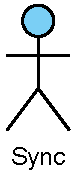
\includegraphics[height=3in]{imgs/gruppo1/Attore-Sync.pdf}
\end{center}

%%%%%%%%%%%%%%%%%% 8.1.2 Studente %%%%%%%%%%%%%%%%
\subsection{Studente}
\paragraph{} 
Studente regolarmente iscritto all’\textit{Università degli Studi Del Molise}, munito delle credenziali per accedere al portale dello studente \textit{Esse3}, il servizio esterno sul quale si basa l’applicazione. Lo studente utilizza l’applicazione per usufruire in maniera agevole dei servizi offerti dai portali dell’\textit{Università degli Studi del Molise} e monitorare la propria carriera universitaria.
\begin{center}
	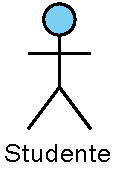
\includegraphics[height=3in]{imgs/gruppo1/Attore-Studente.pdf}
\end{center}

\section{Scenari}

%%%%%%%%%%%%%%%%%% 8.4.1 Visualizza corsi %%%%%%%%%%%%%%%%
\subsection{Visualizza corsi}
\paragraph{Visualizzazione avvenuta con successo.} 
Lo studente Giuseppe, iscritto al terzo anno della facoltà di Informatica, accede alla sezione \textit{Piano di studio} per visualizzare i corsi del piano di studio. Nello specifico, per ogni corso il sistema mostra il nome e, se superato, il voto e la data di verbalizzazione:

\begin{tabbing}
	%La prima righa non viene stampata, serve solo per la spaziatura
	\hspace{1cm}-----------------Esame--------------------------- \= --Voto--- \= --------Data------ \kill
	%Scrivere da qui
	\hspace{1cm} • Programmazione e laboratorio \> 25 \> 01/07/2018 \\
	\hspace{1cm} • Architettura degli elaboratori \> 28 \> 21/01/2018 \\
	\hspace{1cm} • Informatica giuridica \> 30 \> 07/06/2018 \\
	\hspace{1cm} • Matematica \> 24 \> 20/07/2018 \\
	\hspace{1cm} • Basi di dati e sistemi informativi \> 30 \> 15/07/2019 \\
	\hspace{1cm} • Calcolo numerico \> 18 \> 26/03/2019 \\
	\hspace{1cm} • Storia della matematica \> N/D \>\\
	\hspace{1cm} • Informatica territoriale \> N/D \>\\
	\hspace{1cm} • Statistica \> N/D \>\\
	\hspace{1cm} • Intelligenza artificiale \> N/D \>\\
	\hspace{1cm} • Programmazione mobile \> N/D \>\\
\end{tabbing}

%%%%%%%%%%%%%%%%%% 8.4.2 Ricerca corsi %%%%%%%%%%%%%%%%
\subsection{Ricerca corsi}
\paragraph{Ricerca avvenuta con successo.} 
Lo studente Giuseppe, iscritto al terzo anno della facoltà di Informatica, dopo aver visualizzato i corsi del piano di studio, inserisce la parola chiave \textbf{\textit{“Matematica”}}. Il sistema trova i corsi e mostra i risultati:

\begin{tabbing}
	%La prima righa non viene stampata, serve solo per la spaziatura
	\hspace{1cm}-----------------Esame--------------------------- \= --Voto--- \= --------Data------ \kill
	%Scrivere da qui
	\hspace{1cm} • Matematica \> 24 \> 20/07/2018 \\
	\hspace{1cm} • Storia della matematica \> N/D \>\\
\end{tabbing}

\paragraph{La ricerca non restituisce risultati.} 
Lo studente Giuseppe, iscritto al terzo anno della facoltà di Informatica, dopo aver visualizzato i corsi del piano di studio, inserisce la parola chiave \textbf{\textit{“Matemagica”}}. Il sistema non restituisce alcun riscontro e mostra allo studente il messaggio di errore “Nessun corso trovato”.




\section{Casi d'uso}
\subsection{Visualizza corsi}
Per ogni caso d'uso inserire descrizione e tabella. Se il tuo caso d'uso prevede più attori di quelli che sono nella tabella sottostante di esempio, aggiungi una colonna nella sezione flusso degli eventi!

\paragraph{Caso d'uso 1 (sostituire con nome caso d'uso) \\} 
Lorem ipsum dolor sit amet (sostituire con descrizione caso d'uso)

\begin{table}[tb]
%\normalsize % Dimensione testo normale
\small % Dimensione testo piccola
%\footnotesize % Dimensione testo piccolissima
%\scriptsize % Dimensione del testo ulteriormente più piccola
%\caption{} % Didascalia tabella
%\label{} % Etichetta per riferimenti incrociati
\begin{tabular}{| p{\useCaseLeft} | p{\useCaseNum} | p{\useCaseTwoCol} | p{\useCaseTwoCol} |}
	\hline
	\textbf{Nome caso d'uso} & \multicolumn{3}{p{\useCaseMulticol} |}{\textbf{Login}} \\
	\hline
	\textbf{Attori partecipanti} & \multicolumn{3}{p{\useCaseMulticol} |}{Inizializzato da \textbf{Utente}.} \\
	\hline
	\textbf{Condizioni d'ingresso} & \multicolumn{3}{p{\useCaseMulticol} |}{L'utente ha cliccato sul bottone di login.} \\
	\hline
	\textbf{Flusso degli eventi} & \textbf{\#} & \textbf{Utente} & \textbf{Sistema} \\
	\hline
	\textbf{} & \textbf{1} & \textbf{} & Propone una schermata per l'inserimento dei dati necessari per il login, e-mail e password dell'utente \\
	\hline
	\textbf{} & \textbf{2} & Inserisce i dati e sottomette la richiesta & \textbf{} \\
	\hline
	\textbf{} & \textbf{3} & \textbf{} & Controlla che siano stati inseriti entrambi i campi e avvia le operazioni di visualizzazione \\
	\hline
	\textbf{Eccezioni} & \multicolumn{3}{p{\useCaseMulticol} |}{3.1 Uno o entrambi i campi sono vuoti.\newline 3.2 Le credenziali inserite non sono valide (una o entrambe).} \\
	\hline
	\textbf{Condizioni d'uscita} & \multicolumn{3}{p{\useCaseMulticol} |}{Il sistema completa la login e dà accesso all'app o, in caso contrario, visualizza un messaggio di errore se non sono stati inseriti tutti i dati obbligatori, se le credenziali non sono corrette o se si verifica un insuccesso dell'operazione.} \\
	\hline
\end{tabular}
\end{table}

\section{Diagramma dei casi d'uso}

Inserire immagine del diagramma. Le immagini vanno caricate nella cartella imgs, va inserito il path corrispondente (nomefile.estensione) dopo il tag includegraphics e va cambiata la descrizione dell'immagine (caption) con un'etichetta opportuna. Sostituire l'immagine file-comuni-ai-gruppi/useCaseEsempio.png con quella desiderata.

\begin{figure}
	\centering
	\includegraphics[height=3in]{imgs/file-comuni-ai-gruppi/useCaseEsempio.png}
	\caption{Inserire descrizione}
	\label{fig:prova}
\end{figure}

\section{Diagramma di sequenza}

Inserire immagine del diagramma. Le immagini vanno caricate nella cartella imgs, va inserito il path corrispondente (nomefile.estensione) dopo il tag includegraphics e va cambiata la descrizione dell'immagine (caption) con un'etichetta opportuna. Sostituire l'immagine file-comuni-ai-gruppi/useCaseEsempio.png con quella desiderata.

\begin{figure}
	\centering
	\includegraphics[height=3in,width=5in]{imgs/file-comuni-ai-gruppi/SequenceDgEsempio.png}
	\caption{Inserire descrizione}
	\label{fig:prova}
\end{figure}

\section{Diagramma delle attività}

Inserire immagine del diagramma. Le immagini vanno caricate nella cartella imgs, va inserito il path corrispondente (nomefile.estensione) dopo il tag includegraphics e va cambiata la descrizione dell'immagine (caption) con un'etichetta opportuna. Sostituire l'immagine file-comuni-ai-gruppi/useCaseEsempio.png con quella desiderata.

\begin{figure}
	\centering
	\includegraphics[height=3in,width=5in]{imgs/file-comuni-ai-gruppi/ActivityDgEsempio.png}
	\caption{Inserire descrizione}
	\label{fig:prova}
\end{figure}

\clearpage
